% !TEX root = ../main.tex
\documentclass[../main.tex]{subfiles}

\begin{document}
\section{Applications and packages}

\subsection{Tooling}

To run the application and install dependencies the following tools were used:

\begin{itemize}
  \item \textbf{Node.js} \cite{nodejs} - JavaScript runtime environment (v20.10.0)
  \item \textbf{pnpm} \cite{pnpm} - Node.js package manager (v8.6.10)
\end{itemize}

Both tools were installed and managed using \texttt{rtx} \cite{rtx} tool manager.
This tool allows installing and manage many development tools which include Node.js and pnpm.
After navigating to the project directory, rtx will automatically install all tools and select the correct versions based on the \texttt{.rtx.toml}.

\begin{listing}[H]
  \tomlfile{implementation/code/rtx.toml}
  \caption{rtx configuration file used in the project}
\end{listing}

As of writing this document the \textbf{rtx} tool undergoes name change to \textbf{mise}, it will be referred to as \textbf{rtx} in this document.

\subsection{Applications structure}

\begin{figure}[H]
  \centering
  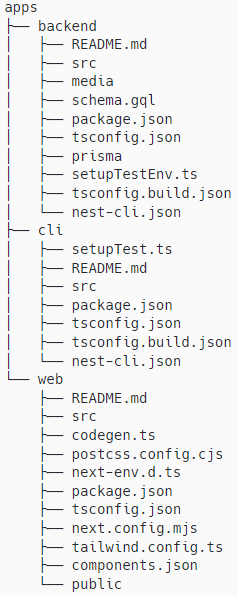
\includegraphics{file-tree/apps.png}
  \caption{Applications file tree (two levels deep)}
  \label{fig:apps-file-tree}
\end{figure}

The web application is a \texttt{Next.js} application and is located in the \texttt{apps/web} directory.
The sources for the \texttt{Next.js} application are located in the \texttt{apps/web/src} directory.
Both the \texttt{backend} and \texttt{cli} are \texttt{NestJS} application and are located in the \texttt{apps/backend} and \texttt{apps/cli} directories respectively.
Thier's sources are also contained in the \texttt{src} directories.

\subsection{Packages structure}

\begin{figure}[H]
  \centering
  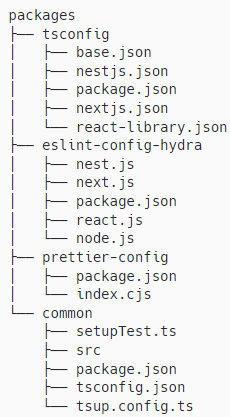
\includegraphics{file-tree/packages.png}
  \caption{Packages file tree (two levels deep)}
  \label{fig:packages-file-tree}
\end{figure}

The \texttt{packages} directory contains all the shared code used in the project.
The \texttt{packages/common} directory contains all the shared code used in the \texttt{backend}, \texttt{cli} and \texttt{web} applications.
Other packages from figure \ref{fig:packages-file-tree} are used to provide the same configuration settings to all application in the \texttt{apps} directory.

As the \textbf{common} is a TypeScript package, it needs to be compiled to JavaScript first before it can be used in the applications.
For this purpose a tool called \texttt{tsup} \cite{tsup} is used which is a TypeScript module bundler.
It transpiles the TypeScript code to JavaScript using \texttt{esbuild} \cite{esbuild} and then bundles each defined module into a single file.
Additionally, it invokes \texttt{tsc} to generate type definitions (\texttt{.d.ts} files \cite{typescript-d-ts}) for the bundled modules.
The \texttt{tsup} tool is configured using the \texttt{tsup.config.ts} file.

\begin{listing}[H]
  \tsfile{implementation/code/tsup.config.ts}
  \caption{tsup configuration file used in the \textbf{common} package}
  \label{code:tsup-config}
\end{listing}

By default, imports are possible only using package name as an import specifier as shown in listing \ref{code:import-package-name},
which would be \texttt{@hydra-ipxe/common} in the case of the \textbf{common} package.

\begin{listing}[H]
  \begin{tscode}
    import { someFunc } from '@hydra-ipxe/common';
  \end{tscode}
  \caption{Importing functions using package name as import specifier}
  \label{code:import-package-name}
\end{listing}

The file defined in the \texttt{main} field of the \texttt{package.json} file is used as the entry point for the package.
By default, this file is the \texttt{index.js} file, which is the default entry point for Node.js packages.

This means that every function that would be used by the applications would have to be exported from the \texttt{index.js} file.
This would lead to a very large file which would be hard to maintain and navigate. Bundlers can also struggle to remove unused code in a process called tree shaking \cite{tree-shaking}.
To avoid this problem, the \texttt{exports} field in the \texttt{package.json} file is used to define the entry points for the package.
There the rules for resolving the imports specifies are defined. As currently there are many different module formats used for the JavaScript module system,
the exports' system can be also used to determinate which files should be used for each module format. The project uses \texttt{ESM} \cite{esm} module format for frontend code and \texttt{CJS} \cite{cjs} for backend code.
This is reflected in the \texttt{format} field in the \texttt{tsup} configuration file (listing \ref{code:tsup-config}).

\begin{listing}[H]
  \jsonfile{implementation/code/package-exports.jsonc}
  \caption{Exports configuration file used in the \textbf{common} package}
  \label{code:package-exports}
\end{listing}

The rules defined in the \texttt{exports} field are used to resolve the import specifiers. Which allows importing individual files from the \texttt{common} package.

\begin{listing}[H]
  \begin{tscode}
    import {
    BasicBootDataSchema,
    type IPXEStrategy,
    } from '@hydra-ipxe/common/shared/ipxe/strategies.def';
  \end{tscode}
  \caption{Example import, importing individual files from the \textbf{common} package. This is allowed due to the \texttt{exports} field as shown in listing \ref{code:package-exports}}
\end{listing}

\subsection{Service containers}

The \texttt{backend} application requires a \texttt{PostgreSQL} database and a \texttt{Redis} instance to run.
These services are provided using \texttt{Docker} containers, defined in the \texttt{compose.yml} file.
Docker compose \cite{docker-compose} is used to manage the containers and their configuration.

\begin{listing}[H]
  \yamlfile{implementation/code/compose.yml}
  \caption{Docker compose configuration file}
\end{listing}

The values for database user and password are taken from the environment with predefined value if not set.


\end{document}